Deemos realizar un manejo eficiente de la base de datos de \emph{Rededit}. Analicemos la estructura del razonamiento que 
nos lleva a usar \emph{Haas} como una de las mejores alternativas para cumplir con este objetivo:

~

\begin{figure}[!h]
	\begin{center}
		  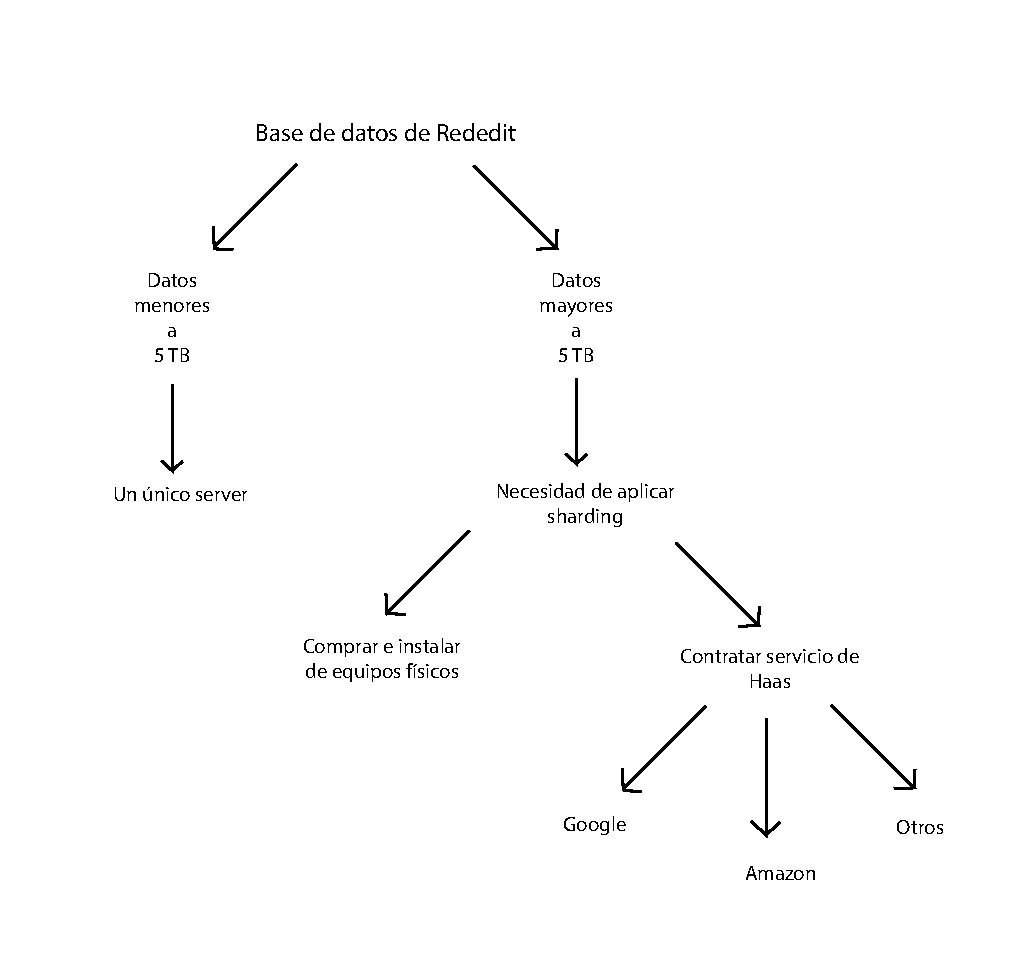
\includegraphics[keepaspectratio]{imagenes/im_1.pdf}
		  \caption{Cada nuevo par de juntas introduce 4 nuevas fuerzas}
		  \label{fig:contra1}
	\end{center}
\end{figure}
\FloatBarrier

\subsection{Sharding, conceptos generales}

''Sharding is the process of storing data records across multiple machines and is MongoDB’s approach to meeting the
demands of data growth. As the size of the data increases, a single machine may not be sufficient to store the data nor
provide an acceptable read and write throughput. Sharding solves the problem with horizontal scaling. With sharding,
you add more machines to support data growth and the demands of read and write operations.'' (MongoDB-sharding-guide)

''Vertical scaling adds more CPU and storage resources to increase capacity. Scaling by adding capacity has lim-
itations: high performance systems with large numbers of CPUs and large amount of RAM are disproportionately
more expensive than smaller systems. Additionally, cloud-based providers may only allow users to provision smaller
instances. As a result there is a practical maximum capability for vertical scaling.'' (MongoDB-sharding-guide)

''Sharding, or horizontal scaling, by contrast, divides the data set and distributes the data over multiple servers, or
shards. Each shard is an independent database, and collectively, the shards make up a single logical database.''

\subsection{Sharding en MongoDB}

MongoDB soporta sharding a través de estructuras llamadas \emph{sharded clusters},
que cuentan con los siguientes componentes:

\begin{itemize}
	\item Shards o \emph{mongod}
	\item Query routers o \emph{mongos}
	\item Config servers 
\end{itemize}


\subsection{Decisiones de arquitectura}

Para establecer la base de datos de \emph{Rededit} tomamos las siguientes decisiones de arquitectura:

\subsubsection{\emph{Replica set}}

Cada \emph{shard} está constituido por un \emph{replica set}: un conjunto de procesos \emph{mongod} que mejoran la 
disponibilidad de los datos del
servidor en base a la redundancia. Existen tres tipos de miembros:

\begin{description}
	\item[Primario] Recibe las operaciones de escritura.
	\item[Secundario] Replican las mismas operaciones efectuadas por el primario para mantener el set de datos consistente.
	\item[Árbitro] Opcional. 
	No almacena datos. Simplemente participa en la elección de un nuevo nodo primario en los casos en donde el actual se
	encuentra inhabilitado.
\end{description}

Decidimos adoptar una de las configuraciones típicas que propone \emph{MongoDB-replication-guide}: 
Una estructura conformada por tres nodos, todas ellas almacenando datos: 

\begin{description}
	\item[Uno primario] 
	\item[Dos secundarios] Ambos son candidatos a volverse primarios luego de una elección, en el caso de una falla
	en el nodo primario.
	\item[Ningún árbitro]
\end{description}

Mediante esta elección disponemos de 2 copias completas del set de datos además del primario. Provee tolerancia a fallos
en el nodo primario, y buena velocidad de respuesta debido a la redundancia.








